\subsection{Søking}
\begin{frame}[fragile]{Søking}
    Big O er pessimistisk, og bryr seg kun om det verste tenkelige tilfellet.
    \begin{minted}[fontsize=\scriptsize]{python}
def index_of(list, e):
    for i in range(len(list)): # O(n)
        if list[i] == e:       # O(1)
            return i           # O(1)
    return -1                  # Total: O(n)
    \end{minted}
    Summen er fortsatt $O(n)$, selv om det er mulig vi blir ferdig tidligere.
\end{frame}

\begin{frame}[fragile]{Binærsøk}
    \begin{columns}
        \begin{column}{0.50\textwidth}
            \begin{figure}
                \centering
                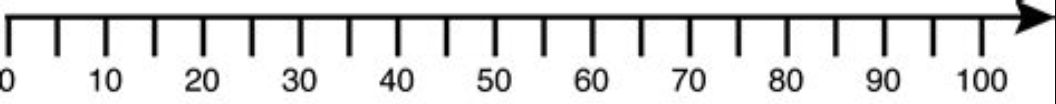
\includegraphics[scale=0.3]{images/Tallinje.png}
                \label{fig:tall}
            \end{figure}  
            \pause
            \begin{minted}[fontsize=\scriptsize]{python}
def binary_search(list, target):
    left = 0
    right = len(arr) - 1
    while left <= right:
        mid = (left + right) // 2
        if arr[mid] == target: return mid
        elif arr[mid] < target: left = mid + 1
        else: right = mid - 1
    return -1
            \end{minted}       
        \end{column}
        \begin{column}{0.47\textwidth}
            Hvor mange operasjoner blir det?\\\pause
            Vi må finne ut hvor mange ganger løkken looper.\\\pause
            I hver iterasjon blir avstanden mellom $left$ og $right$ halvert, og det kan gjøres $log_2(n)$ ganger før vi kommer til 0 eller 1.\\[2mm]\pause
            Dermed kjører binærsøk i $log_2(n)$, som er veldig mye bedre enn $O(n)$.
        \end{column}
    \end{columns}
\end{frame}